\documentclass[a4paper, 12pt]{article}
% packages
\usepackage{amssymb}
\usepackage[fleqn]{mathtools}
\usepackage{tikz}
\usepackage{enumerate}
\usepackage{bussproofs}
\usepackage{xcolor}
\usepackage[margin=1.3cm]{geometry}
\usepackage{logicproof}
\usepackage{diagbox}
\usepackage{listings}
\usepackage{graphicx}
\usepackage{lstautogobble}
\usepackage{hyperref}
\usepackage{multirow}
\usepackage{tipa}
\usetikzlibrary{decorations.pathreplacing, arrows, shapes.gates.logic.US, circuits.logic.US, calc, automata, positioning, intersections}

% shorthand for verbatim
% this clashes with logicproof, so maybe fix this at some point?
\catcode`~=\active
\def~#1~{\texttt{#1}}

% code listing
\lstdefinestyle{main}{
    numberstyle=\tiny,
    breaklines=true,
    showspaces=false,
    showstringspaces=false,
    tabsize=2,
    numbers=left,
    basicstyle=\ttfamily,
    columns=fixed,
    fontadjust=true,
    basewidth=0.5em,
    autogobble,
    xleftmargin=3.0ex,
    mathescape=true
}
\newcommand{\dollar}{\mbox{\textdollar}} %
\lstset{style=main}

% augmented matrix
\makeatletter
\renewcommand*\env@matrix[1][*\c@MaxMatrixCols c]{%
\hskip -\arraycolsep
\let\@ifnextchar\new@ifnextchar
\array{#1}}
\makeatother

% ceiling / floor
\DeclarePairedDelimiter{\ceil}{\lceil}{\rceil}
\DeclarePairedDelimiter{\floor}{\lfloor}{\rfloor}

% custom commands
\newcommand{\indefint}[2]{\int #1 \, \mathrm{d}#2}
\newcommand{\defint}[4]{\int_{#1}^{#2} #3 \, \mathrm{d}#4}
\newcommand{\pdif}[2]{\frac{\partial #1}{\partial #2}}
\newcommand{\dif}[2]{\frac{\mathrm{d}#1}{\mathrm{d}#2}}
\newcommand{\limit}[2]{\raisebox{0.5ex}{\scalebox{0.8}{$\displaystyle{\lim_{#1 \to #2}}$}}}
\newcommand{\summation}[2]{\sum\limits_{#1}^{#2}}
\newcommand{\product}[2]{\prod\limits_{#1}^{#2}}
\newcommand{\intbracket}[3]{\left[#3\right]_{#1}^{#2}}
\newcommand{\ulsmash}[1]{\underline{\smash{#1}}}

\newcommand{\powerset}[0]{\wp}
\renewcommand{\emptyset}[0]{\varnothing}

\makeatletter
\newsavebox{\@brx}
\newcommand{\llangle}[1][]{\savebox{\@brx}{\(\m@th{#1\langle}\)}%
  \mathopen{\copy\@brx\kern-0.5\wd\@brx\usebox{\@brx}}}
\newcommand{\rrangle}[1][]{\savebox{\@brx}{\(\m@th{#1\rangle}\)}%
  \mathclose{\copy\@brx\kern-0.5\wd\@brx\usebox{\@brx}}}
\makeatother
\newcommand{\lla}{\llangle}
\newcommand{\rra}{\rrangle}
\newcommand{\la}{\langle}
\newcommand{\ra}{\rangle}
\newcommand{\crnr}[1]{\text{\textopencorner} #1 \text{\textcorner}}
\newcommand{\laplace}{\mathcal{L}}
\newcommand{\fourier}{\mathcal{F}}

\newcommand{\mat}[1]{\boldsymbol{#1}}
\renewcommand{\vec}[1]{\boldsymbol{#1}}
\newcommand{\rowt}[1]{\begin{bmatrix}
    #1
\end{bmatrix}^\top}

\newcommand{\unaryproof}[2]{\AxiomC{#1} \UnaryInfC{#2} \DisplayProof}
\newcommand{\binaryproof}[3]{\AxiomC{#1} \AxiomC{#2} \BinaryInfC{#3} \DisplayProof}
\newcommand{\trinaryproof}[4]{\AxiomC{#1} \AxiomC{#2} \AxiomC{#3} \TrinaryInfC{#4} \DisplayProof}

\newcommand{\axiom}[1]{\AxiomC{#1}}
\newcommand{\unary}[1]{\UnaryInfC{#1}}
\newcommand{\binary}[1]{\BinaryInfC{#1}}
\newcommand{\trinary}[1]{\TrinaryInfC{#1}}
\newcommand{\quaternary}[1]{\QuaternaryInfC{#1}}
\newcommand{\quinary}[1]{\QuinaryInfC{#1}}
\newcommand{\dproof}[0]{\DisplayProof}

\newcommand{\bnfsep}[0]{\ |\ }
\newcommand{\lrbt}[0]{\ \bullet\ }
\newcommand{\concsep}[0]{\ ||\ }
\newcommand{\ttbs}{\char`\\}

\newcommand{\violet}[1]{\textcolor{violet}{#1}}
\newcommand{\blue}[1]{\textcolor{blue}{#1}}
\newcommand{\red}[1]{\textcolor{red}{#1}}

% no indent
\setlength\parindent{0pt}

% reasoning proofs
\usepackage{ltablex}
\usepackage{environ}
\keepXColumns
\NewEnviron{reasoning}{
    \begin{tabularx}{\textwidth}{rlX}
        \BODY
    \end{tabularx}
}
\newcommand{\proofline}[3]{$(#1)$ & $#2$ & \hfill #3 \smallskip \\}
\newcommand{\proofarbitrary}[1]{& take arbitrary $#1$ \smallskip \\}
\newcommand{\prooftext}[1]{\multicolumn{3}{l}{#1} \smallskip \\}
\newcommand{\proofmath}[3]{$#1$ & = $#2$ & \hfill #3 \smallskip \\}
\newcommand{\prooftherefore}[1]{& $\therefore #1$ \smallskip \\}
\newcommand{\proofbc}[0]{\prooftext{\textbf{Base Case}}}
\newcommand{\proofis}[0]{\prooftext{\textbf{Inductive Step}}}

% reasoning er diagrams
\newcommand{\nattribute}[4]{
    \node[draw, state, inner sep=0cm, minimum size=0.2cm, label=#3:{#4}] (#1) at (#2) {};
}
\newcommand{\mattribute}[4]{
    \node[draw, state, accepting, inner sep=0cm, minimum size=0.2cm, label=#3:{#4}] (#1) at (#2) {};
}
\newcommand{\dattribute}[4]{
    \node[draw, state, dashed, inner sep=0cm, minimum size=0.2cm, label=#3:{#4}] (#1) at (#2) {};
}
\newcommand{\entity}[3]{
    \node[] (#1-c) at (#2) {#3};
    \node[inner sep=0cm] (#1-l) at ($(#1-c) + (-1, 0)$) {};
    \node[inner sep=0cm] (#1-r) at ($(#1-c) + (1, 0)$) {};
    \node[inner sep=0cm] (#1-u) at ($(#1-c) + (0, 0.5)$) {};
    \node[inner sep=0cm] (#1-d) at ($(#1-c) + (0, -0.5)$) {};
    \draw
    ($(#1-c) + (-1, 0.5)$) -- ($(#1-c) + (1, 0.5)$) -- ($(#1-c) + (1, -0.5)$) -- ($(#1-c) + (-1, -0.5)$) -- cycle;
}
\newcommand{\relationship}[3]{
    \node[] (#1-c) at (#2) {#3};
    \node[inner sep=0cm] (#1-l) at ($(#1-c) + (-1, 0)$) {};
    \node[inner sep=0cm] (#1-r) at ($(#1-c) + (1, 0)$) {};
    \node[inner sep=0cm] (#1-u) at ($(#1-c) + (0, 1)$) {};
    \node[inner sep=0cm] (#1-d) at ($(#1-c) + (0, -1)$) {};
    \draw
    ($(#1-c) + (-1, 0)$) -- ($(#1-c) + (0, 1)$) -- ($(#1-c) + (1, 0)$) -- ($(#1-c) + (0, -1)$) -- cycle;
}

% actual document
\begin{document}
    \section*{CO211 - Operating Systems}
        \subsection*{4th October 2019}
            \subsubsection*{Outline of the Course}
                \begin{itemize}
                    \itemsep0em
                    \item overview and introduction \hfill structure, case studies
                    \item processes and threads \hfill abstractions that an OS uses to execute code
                    \item inter-process communication (IPC) \hfill allows multiple processes to communicate with each other
                    \item memory management \hfill allocation, abstraction for virtual memory, paging
                    \item device management \hfill types, drivers
                    \item disk management \hfill scheduling, caching, RAID
                    \item file systems \hfill basic abstractions for storage and implementation
                    \item security \hfill authentication, access control
                \end{itemize}
                Note that this follows a similar structure to most OS courses, and therefore we can reference content from other sources.
                \textit{Operating Systems: Three Easy Pieces} is recommended, as it bridges between this course and the PintOS lab.
            \subsubsection*{Overview}
                The general overview is that there is a system bus that interconnects different hardware components (including CPU and memory), and allows for communication between them.
                \medskip

                The operating system provides abstractions for programs to use, meaning that they do not have to deal with the complex hardware.
                For example, a process abstraction expects an interface to the hardware, which allows programs to be used on different hardware.
                This means that the OS will need how to to control the hardware with drivers.
                The operating system has the following goals;
                \begin{enumerate}[(1)]
                    \itemsep0em
                    \item \textbf{managing resources}
                        \medskip

                        The operating system must be able to expose the resources efficiently to the application, and also share these resources fairly.
                        Some examples are;
                        \begin{itemize}
                            \itemsep0em
                            \item CPU (multiple cores) \hfill should decide what runs on each hardware thread
                            \item memory \hfill cache, RAM
                            \item I/O devices \hfill displays (GPUs), network interfaces
                            \item internal devices \hfill clocks, timers, interrupt controllers
                            \item persistent storage
                        \end{itemize}
                        OS uses both time and space multiplexing for sharing.
                        An example for the former is how the effect of parallelism can be achieved with a single CPU core by splitting up the time allocated per process, and an example for the latter is splitting up memory for each process.
                        \smallskip

                        On the other hand, with allocation, the OS must also support simultaneous resource access (such as to disks, RAM, network etc.).
                        Continuing from this, it must also offer mutual exclusion, thus protecting risky operations (such as file writing).
                        Generally, the OS aims to protect against corruption.
                        \smallskip

                        Finally, the operating system must also handle storing data, and enforce access control.
                    \item \textbf{clean interfaces}
                        \medskip

                        The OS should hide away the hardware, and applications use the hardware through an interface provided by the operating system.
                        We can think of this as a virtual machine abstraction on top of the bare machine - similar to how the JVM works (but at a lower layer).
                    \item \textbf{concurrency and non-determinism}
                        \medskip

                        The operating system must be able to deal with concurrency, for example overlapping I/O and computation.
                        This is because I/O devices tend to be slower, and while the device is working on the task, it shouldn't prevent the CPU from doing other work.
                        An operating system may switch activities at arbitrary times, and this must be done safely - by offering synchronisation primitives.
                        It should also protect processes by giving each program its own space, thus preventing interference.
                        \smallskip

                        Similarly, the OS is fundamentally non-deterministic, as it needs to handle interrupts (such as the network card receiving a packet, user interrupts, etc.).
                \end{enumerate}
            \subsubsection*{Tutorial Questions}
                \begin{enumerate}[1)]
                    \itemsep0em
                    \item List the most important resources that must be managed by an operating system in the following settings;
                        \begin{enumerate}[(a)]
                            \itemsep0em
                            \item supercomputer
                                \begin{itemize}
                                    \itemsep0em
                                    \item computation time \hfill primarily used for intensive computations
                                    \item memory
                                \end{itemize}
                            \item networked workstations connected to a server
                                \begin{itemize}
                                    \itemsep0em
                                    \item bandwidth \hfill must handle packet processing and network traffic
                                \end{itemize}
                            \item smartphone
                                \begin{itemize}
                                    \itemsep0em
                                    \item energy \hfill limited power, can power off unused hardware
                                    \item mobile network \hfill (including other communication technology)
                                    \item other sensors \hfill issues of privacy, when to expose GPS etc.
                                \end{itemize}
                        \end{enumerate}
                        As this highlights, some uses will need specially designed operating systems.
                        We also have general-process OS, as it takes a large amount of effort to implement a new operating system.
                    \item What is the \textbf{kernel} of an operating system?
                        \medskip

                        The part of the OS is always in memory, and runs in the privileged part of the CPU (user mode cannot access all functionality).
                        Implements commonly used functions of the OS and has complete access to all hardware.
                \end{enumerate}
            \subsubsection*{Kernel Design}
                \begin{itemize}
                    \itemsep0em
                    \item \textbf{monolithic kernel}
                        \medskip

                        Consider it as one large program that has all the functionality that you want an OS to perform.
                        \smallskip

                        The kernel is a single executable with its own address space.
                        There exists a \textbf{system call} interface that allows user mode applications to access the hardware.
                        Software invokes functionality from the kernel by issuing system calls - the CPU must switch from user mode to kernel mode to support this.
                        The kernel then executes some instruction on behalf of the application.
                        Device drivers are part of the monolithic kernel.
                        \begin{center}
                            \begin{minipage}[t]{0.45\textwidth}
                                advantages
                                \begin{itemize}
                                    \itemsep0em
                                    \item efficient calls within the kernel, as there it remains in kernel mode
                                    \item flexible to write kernel components due to the shared memory (direct access with no limit to APIs)
                                \end{itemize}
                            \end{minipage}
                            \hfill
                            \begin{minipage}[t]{0.45\textwidth}
                                disadvantages
                                \begin{itemize}
                                    \itemsep0em
                                    \item complex design
                                    \item no protection between bits of kernel functionality, therefore any bugs within the kernel will crash the entire machine
                                \end{itemize}
                            \end{minipage}
                        \end{center}
                    \item \textbf{microkernels}
                        \medskip

                        Only includes functionality that \textbf{requires} direct access to the hardware (or to be run in kernel mode).
                        This is a minimalistic design and has the advantage of fewer bugs (due to the smaller amount of code).
                        \begin{center}
                            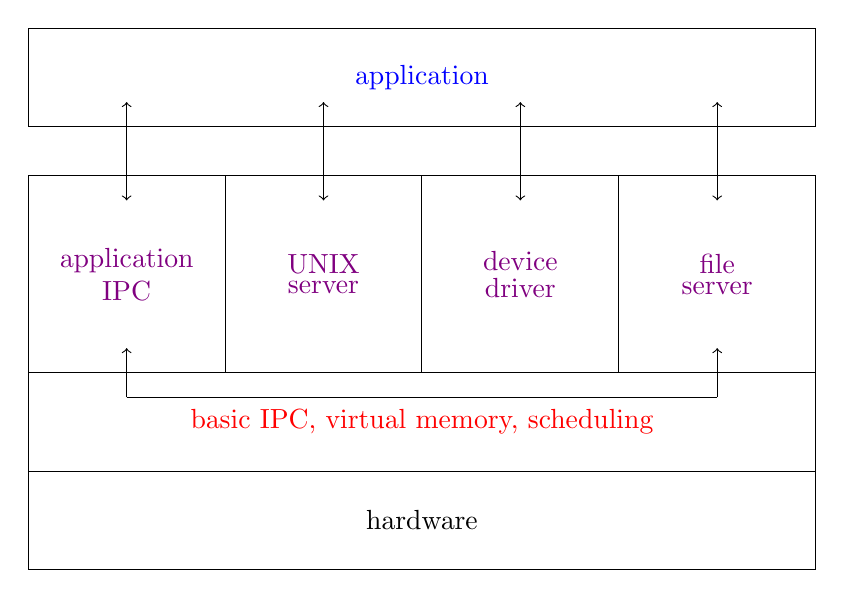
\begin{tikzpicture}[x=2.5cm, y=1.25cm]
                                \node[blue] at (2, -0.5) {application};
                                \node[violet] at (0.5, -2.5) {\shortstack{application\\IPC}};
                                \node[violet] at (1.5, -2.5) {\shortstack{UNIX\\server}};
                                \node[violet] at (2.5, -2.5) {\shortstack{device\\driver}};
                                \node[violet] at (3.5, -2.5) {\shortstack{file\\server}};
                                \node[red] at (2, -4) {basic IPC, virtual memory, scheduling};
                                \node at (2, -5) {hardware};

                                \draw
                                (0.5, -0.75) edge[<->] (0.5, -1.75)
                                (1.5, -0.75) edge[<->] (1.5, -1.75)
                                (2.5, -0.75) edge[<->] (2.5, -1.75)
                                (3.5, -0.75) edge[<->] (3.5, -1.75)
                                (0.5, -3.75) edge[->] (0.5, -3.25)
                                (3.5, -3.75) edge[->] (3.5, -3.25)
                                (0.5, -3.75) -- (3.5, -3.75);

                                \draw (0, 0) -- (4, 0) -- (4, -1) -- (0, -1) -- cycle;
                                \draw (0, -1.5) -- (4, -1.5) -- (4, -3.5) -- (0, -3.5) -- cycle
                                (1, -1.5) -- (1, -3.5)
                                (2, -1.5) -- (2, -3.5)
                                (3, -1.5) -- (3, -3.5);
                                \draw (0, -3.5) -- (0, -4.5) -- (4, -4.5) -- (4, -3.5);
                                \draw (0, -4.5) -- (0, -5.5) -- (4, -5.5) -- (4, -4.5);
                            \end{tikzpicture}
                        \end{center}
                        Note that both the \blue{application} and \violet{servers} run in user mode, and the \red{kernel} is in kernel mode.
                        The kernel performs IPC between the servers, which are separated for device I/O, scheduling. file access etc.
                        \begin{center}
                            \begin{minipage}[t]{0.45\textwidth}
                                advantages
                                \begin{itemize}
                                    \itemsep0em
                                    \item less complex kernel
                                    \item clean interfaces for the servers
                                    \item more reliable; one of the servers could crash and then restart, without bringing the entire kernel down
                                \end{itemize}
                            \end{minipage}
                            \hfill
                            \begin{minipage}[t]{0.45\textwidth}
                                disadvantages
                                \begin{itemize}
                                    \itemsep0em
                                    \item performance overhead due to the requirement of message passing and transitioning between user mode and kernel mode (checks must be done to maintain the separation) - less of an issue now due to better hardware (e.g \textit{Android})
                                \end{itemize}
                            \end{minipage}
                        \end{center}
                    \item \textbf{hybrid kernel} \hfill many modern designs use a combination of both
                        \medskip

                        This is a more structured design, however user-level servers can incur a performance penalty.
                \end{itemize}
            \subsubsection*{Linux Kernel}
                The structure of Linux system calls is to put arguments into registers Or on the stack, and then issue a trap to switch the CPU from user to kernel mode.
                \medskip

                While C is the dominant language for the Linux kernel, the interrupt handlers are written in assembly, as they are low level pieces of code, and require fast performance (hence a low instruction count).
                Interrupt handlers are the primary means to interact with devices, it initiates dispatching which stops proxies, saves the state, starts the driver and returns.
                \medskip

                Typically, we can split the Linux kernel into three parts;
                \begin{itemize}
                    \itemsep0em
                    \item \textbf{I/O}
                        \medskip

                        One of the design philosophies under UNIX style operating system is to treat everything as a file, and use this file abstraction to expose different resources.
                        Therefore, a lot of I/O resources can be hidden under this virtual file system.
                    \item \textbf{memory management}
                        \medskip

                        Includes virtual memory with paging (and the abstractions associated with that).
                    \item \textbf{process management}
                        \medskip

                        Includes process and thread abstraction, as well as synchronisation and scheduling between them.
                \end{itemize}
                In addition to this, Linux supports dynamically loaded modules into the kernel.
                This support was important as it allowed for the hardware configuration to change (new devices drivers could be loaded into the kernel, without recompiling).
            \subsubsection*{Windows Kernel}
                The NTOS kernel layer implements Windows system call interface.
                This is an example of a hybrid kernel, as programs build on dynamic code libraries (DLLs) - which also make the kernel modular, however the executive servers in the kernel adopted the server model of the microkernel, but still runs in kernel space for the performance benefits.
                At the lower levels, there still exists a microkernel.
                In addition, there is also a hardware abstraction layer (HAL), as this was designed for portability.
                \medskip

                It's also important to note that there are environment subsystems running in user mode allowing for different APIs to be exposed, including Win32, POSIX, and OS/2.
                While the Windows kernel was designed with a lot of flexibility, due to its nature as proprietary software, it only really focused support (until recently) on Win32 (and also Intel in terms of the HAL).
        \subsection*{9th October 2020}
            \subsubsection*{Tutorial Questions}
                \begin{enumerate}[1.]
                    \itemsep0em
                    \item Why is the separation into a user mode and a kernel mode considered good OS design?
                        \medskip

                        Reduce the amount of code running in kernel mode, since a bug in user mode code should not bring down the entire system.
                    \item Which of the following instructions should only be allowed in kernel mode, and why?
                        \begin{enumerate}[(a)]
                            \itemsep0em
                            \item disable all interrupts \hfill only kernel mode
                                \subitem if a user program were to disable interrupts, it would prevent the OS from scheduling processes
                            \item read the time of day clock \hfill not privileged
                            \item change any memory \hfill only kernel mode
                                \subitem typically programs can only access its own memory, such that it cannot accidentally or maliciously interfere with other memory
                            \item set the time of day \hfill typically kernel
                                \subitem most programs assume monotonicity of the clock, and changing to an earlier time can cause bugs
                        \end{enumerate}
                    \item Give an example in which the execution of a user process switches from user mode to kernel mode, and then back to user mode.
                        \medskip

                        Reading a file.
                        Essentially anything that requires a system call, as it requires a switch from user mode to kernel mode, and then back.
                    \item A portable operating system is one that can be ported from one system architecture to another with little modification - explain why it is infeasible to build an OS that is portable without any modification.
                        \medskip

                        At some point in the kernel, it will need to know about the ISA (instruction set architecture) of the CPU (hardware), and what instructions it can support.
                        Some parts of the OS require assembly, and therefore requires modification.
                        The hardware abstraction layer in the Windows kernel makes this easier.
                \end{enumerate}
            \subsubsection*{Processes}
                One of the oldest abstractions in computing.
                This is an instance of a program being executed - this is useful as we can then execute multiple programs "simultaneously" on one processor, especially if not all resources are needed at the same time.
                This provides isolation between programs (own address space), and therefore doesn't interfere with other unrelated processes - if it needs to, then the IPC provided can be used.
                It also makes programming easier, as a programmer can assume it is the only process running.
            \subsubsection*{Concurrency}
                It's important to note that there exists both pseudo-concurrency (on one CPU core), as well as real concurrency (across multiple CPU cores).
                The latter will still use the former per core, as the number of processes is much higher than the number of physical cores.
                In the case of multiple cores, we have to deal with conflicting accesses, whereas in the case with a single core, there is only one process really running at a time.
                \medskip

                One method of creating the illusion of concurrency is time slicing.
                The OS switches the process currently running on the CPU with another runnable process, saving the original process' execution state, and then restoring it after it is switched back.
                Note that a runnable process isn't waiting for input, as we want to minimise the amount of time the CPU is idle.
                We also must ensure that the switching is fair - for example, if process ~A~ has a long execution time, compared to an interactive process ~B~, letting ~A~ run for a long period would cause the interactive process to become unresponsive - therefore the time slice tends to be quite short (how often it lets a process run before switching).
                \begin{enumerate}[1.]
                    \itemsep0em
                    \item If on average a process computes $20\%$ of the time, then with 5 processes, we should have $100\%$ CPU utilisation, right?
                        \medskip

                        Only in the ideal case, when they never wait for I/O at the same time.
                        A better estimate is to look at the probability (assuming independence), with $n$ being the number of processes, and $p$ being the fraction of time a process is waiting for I/O.
                        The probability that all are waiting for I/O would be $p^n$, and therefore the CPU utilisation would be $1 - p^n$.
                    \item How many processes nee to be running to only waste $10\%$ of CPU if they spend $80\%$ waiting for I/O?
                        \begin{center}
                            $1 - 0.8^n = 0.9 \Rightarrow 0.8^n = 0.1 \Rightarrow n = \log_{0.8}(0.1) \approx 10$ concurrent processes
                        \end{center}
                \end{enumerate}
            \subsubsection*{Context Switches}
                A context switch is when the processor switches execution from process ~A~ to process ~B~.
                This is done as part of a scheduling decision.
                With timer interrupts, the currently executing program passes control back to the kernel, which can then make a scheduling decision, changing what is currently running, possibly a different program and performing a context switch.
                This causes the order of execution between processes to become non-deterministic, as these events cannot be pre-determined.
                \medskip

                This needs to be transparent to the process, therefore the state needs to be restored exactly, including anything currently in registers (this is saved by the hardware to the stack, before the hardware invokes the interrupt handler).
                This data is stored in a process descriptor, or a process control block (PCB), kept in the process table.
                The process has its own virtual machine;
                \begin{itemize}
                    \itemsep0em
                    \item own virtual CPU
                    \item own address space (stack, heap, text, data, etc.)
                    \item resources it has access to (open file descriptors, etc.)
                \end{itemize}
                The information in registers (such as the program counter, page table register, stack pointer, etc), the process management information (process ID, parents, etc.), as well as file management information also needs to be stored (root directory, working directory, file descriptors, etc.).
                \medskip

                It's also important to avoid unnecessary context switches as they are expensive, not just from the direct cost of managing state, but also the indirect cost to caching (as the old cache contents are no longer relevant).
                Therefore it has to balance fairness, and the frequency of context switches.
            \subsubsection*{Process Lifecycle}
                Processes are created at the startup of a system, by the request of a user, or through a specific system call by a running process.
                These processes can be foreground processes, that the user interacts with, or background processes that provide services (such as printing or mail) or APIs that can be used by other processes (daemons).
                \medskip

                A process can terminate under these conditions;
                \begin{itemize}
                    \itemsep0em
                    \item normal completion, where the process completes execution
                    \item through a system call (~exit()~ in UNIX or ~ExitProcess()~ in Windows)
                    \item abnormal exit, where the process has run into an error or unhandled exception - this is the importance of user and kernel space separation
                    \item aborted, due to another process overruling its execution (such as killing from terminal)
                    \item never - some processes such as daemons should run infinitely and never terminate (unless an error occurs)
                \end{itemize}
                UNIX allows for a process hierarchy (tree), by running ~init~ (typically), and all processes then form a tree.
                On the other hand, Windows has no notion of hierarchy, and rather the parent of a child process is given a token (a handle) to control it.
                This handle can be passed to another process.
\end{document}
